\section{Auswertung}
\subsection{Bestimmung der Apparatekonstanten}

Bevor die Trägheitsmomente der verschiedenen Körper bestimmt werden können müssen die
Apparatekonstanten bestimmt werden. Das ist zum einen die Winkelrichtgröße D und
das Trägheitsmoment der Drillachse $I_D$.

Die Winkelrichtgröße wird mithilfe der Gleichung (4) bestimmt. Die Kraft wird im Abstand
von $r = \SI{4.3}{\centi\meter} = \SI{4.3e-2}{\meter}$ gemessen.


\begin{table}
  \centering
  \caption{Tabelle mit den Messdaten für die Winkelrichtgröße}
  \begin{tabular}{c c c c}
    \toprule
    $\phi$ in Grad & $\phi$ in rad & $F \, \, \text{in} \, N$ &
    $D \, \, \text{in} \, 10^{-2} N \si{\meter}$ \\
    \midrule
    50 &  $\frac{5\pi}{18}$ & 0.42 & 2.07 \\
    60 &  $\frac{\pi}{3}$ & 0.56 & 2.23 \\
    80 &  $\frac{4\pi}{9}$ & 0.8 & 2.46 \\
    90 &  $\frac{\pi}{2} $ & 0.82 & 2.24 \\
    100 & $\frac{5\pi}{9}$ & 0.96 & 2.37 \\
    120 & $\frac{2\pi}{3}$ & 1.16 & 2.38 \\
    140 & $\frac{7\pi}{9}$ & 1.34 & 2.36 \\
    160 & $\frac{8\pi}{9}$ & 1.54 & 2.37 \\
    180 & $\pi           $ & 1.78 & 2.44 \\
    200 & $\frac{10\pi}{9}$ &   2 & 2.46 \\
    \bottomrule
  \end{tabular}
\end{table}

Der Mittelwert und der zugehörige Fehler der Winkelrichtgrößen wird nun mit
folgenden Gleichungen bestimmt:

\begin{gather}
  \bar{D} = \frac{1}{N} \sum_{i=0}^{N} D_i \\
  \Delta D = \frac{1}{\sqrt{N}\sqrt{N-1}} \sqrt{\sum_{i}(D_i-\bar{D})^2}
\end{gather}

Damit ergibt sich für die Winkelrichtgröße:

\centerline{$D = \num{2.388(39)e-2} Nm$}

Nun muss noch das TräTrägheitsmoment der Drillachse bestimmt werden. Dazu muss
die Gleichung (3) für diesen Fall noch angepasst werden, da sich das gesamte
Trägheitsmoment aus dem der Drillachse und der zwei Massen zusammensetzt:

$I = I_D + 2(I_{zh} + ma^2) = I_D + 2(m \left( \frac{d^2}{16} + \frac{h^2}{12} \right)
ma^2)$

Die geometrischen Abmessungen der beiden Massen sind:

\begin{itemize}
  \item Masse m = \SI{222.5e-3}{\kilo\gram}
  \item Höhe h = \SI{0.03}{\meter}
  \item Durchmesser d = \SI{0.035}{\meter}
\end{itemize}

Damit ergibt sich für das Trägheitsmoment der Massen:

\centerline{$I_{zh} = \SI{3.37e-5}{\kilo\gram\meter\squared}$}

Durch Umformung der Gleichung (3) folgt:

%$ \implies T^2 = 4 \pi^2 \frac{I}{D} = \frac{4\pi^2}{D}(I_D + 2(I_{zh} + ma^2))$\\
\begin{equation}
  T^2 = \frac{8\pi^2m}{D} a^2 + \frac{8\pi^2}{D} I_{zh} + \frac{4\pi^2}{D} I_D
\end{equation}


Das Trägheitsmoment der Drillachse wird nun mit einer Ausgleichsrechnung bestimmt.
Die Ausgleichsrechnung wird mit Python 3.6 durchgeführt.

\begin{table}
  \centering
  \caption{Tabelle mit den Messdaten für das Trägheitsmoment der Drillachse}
  \begin{tabular}{c c c c}
    \toprule
    $T$ in \si{\second} & $a$ in \SI{e-2}{\meter} & $T^2$ in \si{\second\squared} &
    $a^2$ in \SI{e-4}{\meter\squared} \\
    \midrule
    2.32 & 3.5  & 5.38  & 12.25 \\
    2.64 & 5.5  & 6.97  & 30.25 \\
    2.67 & 7.5  & 7.13  & 56.25 \\
    3.16 & 9.5  & 9.99  & 90.25 \\
    3.56 & 12.5 & 12.67 & 156.25 \\
    4.44 & 14.5 & 19.71 & 210.25 \\
    5.09 & 18.5 & 25.91 & 342.25 \\
    5.89 & 20.5 & 34.69 & 420.25 \\
    6.52 & 23.5 & 42.51 & 552.25 \\
    7.4  & 26.5 & 54.76 &  702.25 \\
    \bottomrule
  \end{tabular}
\end{table}

\begin{figure}[H]
  \centering
  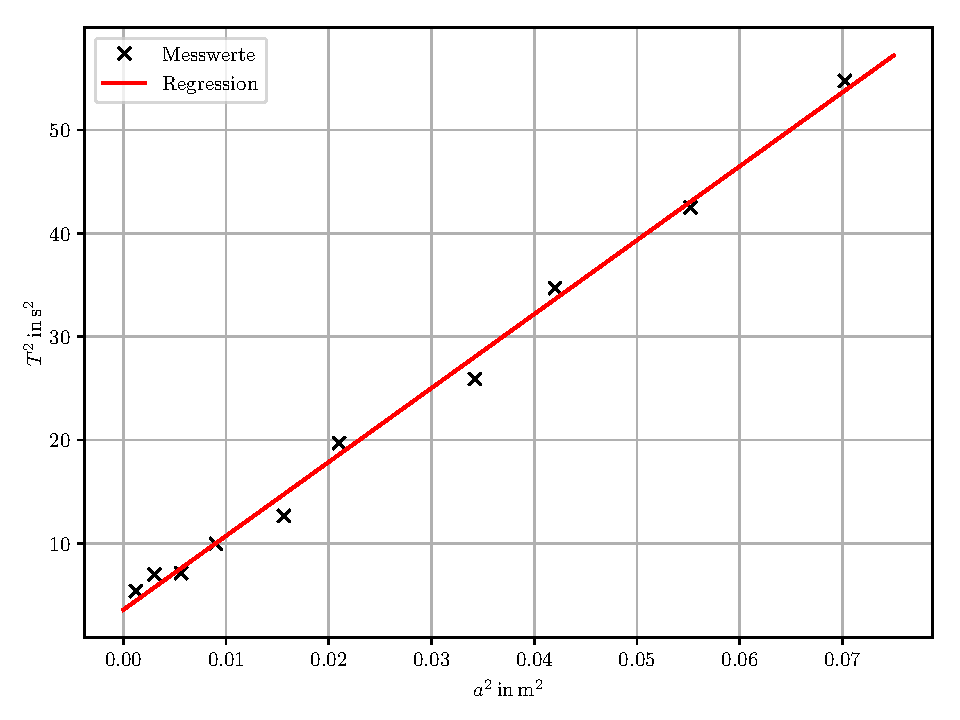
\includegraphics[width=\textwidth]{ausgleichsgerade1.pdf}
  \caption{Graphische Darstellung der Messwerte und der Ausgleichsgeraden}
\end{figure}

Damit ergeben sich die Parameter der Ausgleichsgeraden zu:

\begin{equation}
  y = m'x + b
\end{equation}

\begin{itemize}
  \item $m' = \SI{715.28(1921)}{\kilo\gram\per{\N\meter}}$
  \item $b = \SI{3.571(658)}{\kilo\gram\meter\per\N}$
\end{itemize}

Durch Vergleichen der Gleichungen (7) und (8) lässt sich das Trägheitsmoment der
Drillachse und die Winkelrichtgröße nochmal bestimmen.

\begin{gather}
  D_2 = \frac{8\pi^2m}{m'} \\
  I_D = \frac{D_2}{4\pi^2}b - 2I_{zh}
\end{gather}

Der Fehler der neu bestimmten Winkelrichtgröße wird mit der Gauß`schen Fehlerfortpflanzung
bestimmt:

$\Delta D_2 = \sqrt{\left(\frac{\partial D_2}{\partial m'} \cdot \Delta m' \right)^2}
= \frac{8\pi^2m}{m'^2} \cdot \Delta m'$

Die Winkelrichtgröße ist also:

\centerline{$D_2 = \SI{2.456(66)e-2}{\N\meter}$}

Damit kann nun das Trägheitsmoment der Drillachse bestimmt werden. Der Fehler wird
wieder mit der Gauß´schen Fehlerfortpflanzung bestimmt:

$\Delta I_D = \sqrt{\left(\frac{\partial I_D}{\partial D_2} \cdot \Delta D_2 \right)^2 +
\left(\frac{\partial I_D}{\partial b} \cdot \Delta b \right)^2}$

\centerline{$I_D = \SI{2.154(414)e-3}{\kilo\gram\meter\squared}$}

\subsection{Trägheitsmoment Kugel}
